\biohead{Mary Ellen Moulsdale}{}{}{A portrait taken in Liverpool.\cite{MEMportrait}}

Mary Ellen Moulsdale was born on 4 April 1845 in Liverpool, Lancashire \cite{MEMoulsdaleBirth} and baptised on 24 April 1845 at St Peters Church, Liverpool, Lancashire \cite{MEMoulsdaleBaptism}. Her parents were \bioref{John_Moulsdale} and \bioref{Maria_Jackson} and she had two sisters: Maria Moulsdale (1857--?) and Sarah Ann Moulsdale (1857--?), presumably twins. 

In 1858 she was attending Miss Hawkin's Seminary in Liverpool, Lancashire \cite{MEMoulsdaleSchool}.

By April 1871`she was living at 19 Breck Road, Walton-in-the-Hill with James Denton (at the time aged 66, a Gentleman) and his wife Mary (aged 62) and her sister Maria \cite{MEMoulsdaleResidence}.  She was by then their adopted daughter \cite{MEMoulsdaleAdoption},  but there are no records of why she should have been adopted beyond some personal records made by her husband. 

She married Thomas Henry Barker on 25 August 1875 at St Margarets, in Anfield, Liverpool, Lancashire \cite{MEMoulsdaleMarriage} and they lived at 10 Falkner Street, Liverpool.  They had seven sons: \bioref{James_Denton_Barker}, \bioref{Charles_Frederick_Strangeways_Barker}, Reverend \bioref{Thomas_Percy_Conyers_Barker}, \bioref{Francis_Darcy_Mead_Barker}, \bioref{William_Danby_Holt_Barker}, \bioref{Jonathan_Tong_Barker}, and \bioref{Henry_Bertram_Mitford_Barker}.

She died, aged 91, on 14 December 1936 at 10 Lancaster Avenue, Sefton Park, Merseyside, England \cite{ToxtethBarker20} and the Probate notice read:
``BARKER Mary Ellen of 10 Lancaster Avenue, Sefton Park, Liverpool died 14 December 1936. Probate Liverpool 25 January to James Denton Barker average adjuster. Effects 287 pounds 2 shillings and 4 pence.''

\begin{figure}
 \centering
 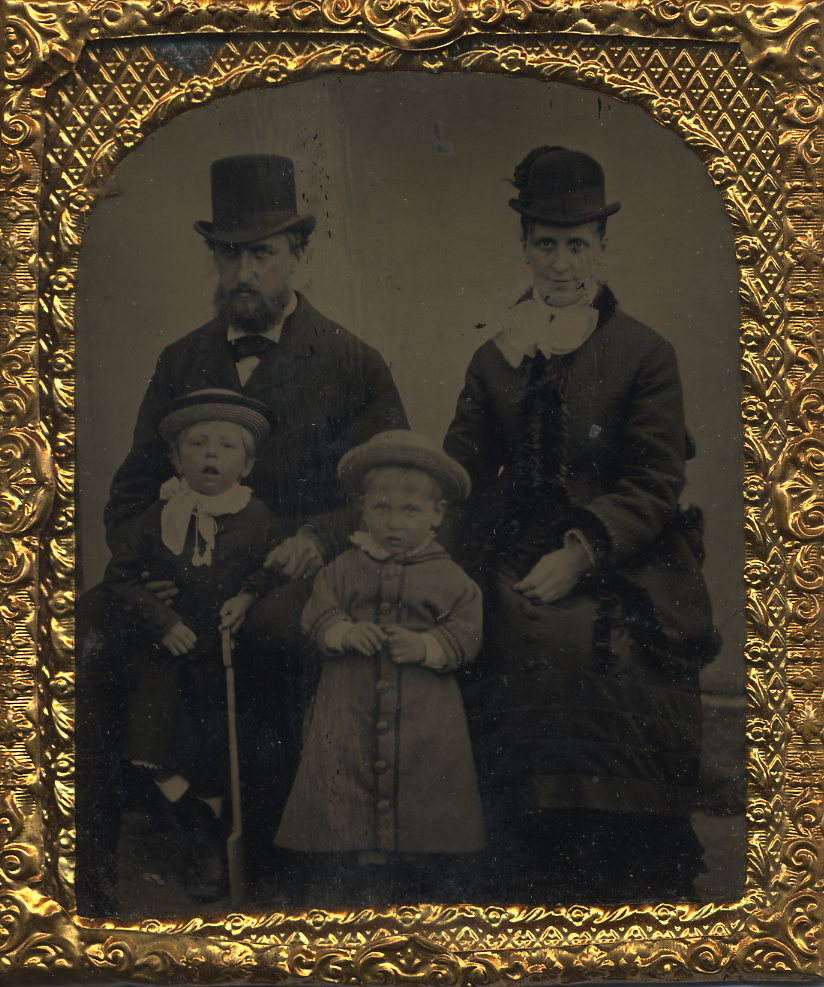
\includegraphics{photos/TH_Barker_with_Mary_Ellen_and_two_children.png}
 \caption{Mary Ellen with her husband and probably \bioref{James_Denton_Barker} and \bioref{Charles_Frederick_Strangeways_Barker}, c.~1880.}
\end{figure}
